% !TEX root = main.tex
\documentclass[12pt, oneside]{article}


%% This template was forked from Winkelmann Template @ OVRLEAF

%%%%%%%%%%%%%%%%%%%%%%%%%%%%
%%   Zusaetzliche Pakete  %%
%%%%%%%%%%%%%%%%%%%%%%%%%%%%
\usepackage[bookmarks]{hyperref}
\usepackage[ngerman]{babel}
\usepackage{acronym} %% I HAVE NO IDEA WHY THERE IS AN ERROR HERE.
\usepackage[T1]{fontenc}
\usepackage[utf8]
{inputenc}
\usepackage{array}
 \usepackage{amsmath}
\usepackage{hyperref}
\usepackage{babel}
\usepackage[T1]{fontenc}
\usepackage{array}
\usepackage{xcolor}
\usepackage{multicol}
\usepackage{hyperref}
\usepackage{tikz}
\usepackage{caption}
\usepackage{enumerate}  
\usepackage{enumitem}
\usepackage{hyperref}
\usepackage{enumitem,amssymb}
\usepackage{enumitem}
\usepackage{a4wide}
\usepackage{fancyhdr}
\usepackage{graphicx}
\usepackage{palatino}
\usepackage{float}
\usepackage{glossaries}
\RequirePackage[ngerman=ngerman-x-latest]{hyphsubst}
\usepackage{listings}
\usepackage[justification=centering, labelfont=bf, textfont=bf]{caption}
\usepackage[a4paper, margin=0cm, left=3cm, top=2.5cm, right=2cm, bottom=3.5cm]{geometry} 
\usepackage{etoolbox}
\usepackage{acronym}
\usepackage{titlesec}
\usepackage[titles]{tocloft}
\usepackage{longtable}
\usepackage{xcolor,colortbl}
\usepackage{pdfpages}
\usepackage[paper=portrait,pagesize]{typearea}
\usepackage[labelfont=bf]{caption} % optional
\usepackage{ragged2e}
\usepackage{lscape}
\usepackage{graphicx}
\usepackage{pdflscape}
\usepackage{fancyhdr}
\usepackage{array}
\usepackage{csquotes}
\usepackage{biblatex}
\usepackage{listings}
\usepackage{xcolor}

\addbibresource{./literature.bib}  
\bibliography{./literature.bib}

%\usepackage{fontspec}

\usepackage{xcolor}

\definecolor{codegreen}{rgb}{0,0.6,0}
\definecolor{codegray}{rgb}{0.5,0.5,0.5}
\definecolor{codepurple}{rgb}{0.58,0,0.82}
\definecolor{backcolour}{rgb}{0.95,0.95,0.92}



\definecolor{codegreen}{rgb}{0,0.6,0}
\definecolor{codegray}{rgb}{0.5,0.5,0.5}
\definecolor{codepurple}{rgb}{0.58,0,0.82}
\definecolor{backcolour}{rgb}{0.95,0.95,0.92}

\lstdefinestyle{mystyle}{
    backgroundcolor=\color{backcolour},   
    commentstyle=\color{codegreen},
    keywordstyle=\color{magenta},
    numberstyle=\tiny\color{codegray},
    stringstyle=\color{codepurple},
    basicstyle=\ttfamily\footnotesize,
    breakatwhitespace=false,         
    breaklines=true,                 
    captionpos=b,                    
    keepspaces=true,                 
    numbers=left,                    
    numbersep=5pt,                  
    showspaces=false,                
    showstringspaces=false,
    showtabs=false,                  
    tabsize=2
}
\lstset{style=mystyle}


\setlength\cftparskip{-2pt}
\setlength\cftbeforesecskip{0pt}
\setlength\cftaftertoctitleskip{0pt}

\DeclareCaptionFormat{myformat}{\fontsize{10}{0}\selectfont#1#2#3}
\captionsetup{format=myformat}

\setlength\parindent{0pt}
\setlength{\parskip}{6pt}
\setlength{\headheight}{0.8cm}

\linespread{1.25}

%\setlength{\cftbeforesecskip}{1.75pt}

\renewcommand{\cftfigpresnum}{Abbildung }
\renewcommand{\cfttabpresnum}{Tabelle }

\renewcommand{\cftfigaftersnum}{:}
\renewcommand{\cfttabaftersnum}{:}

\setlength{\cftfignumwidth}{2.75cm}
\setlength{\cfttabnumwidth}{2cm}

\setlength{\cftfigindent}{0cm}
\setlength{\cfttabindent}{0cm}

\renewcommand{\figurename}{Abbildung}
\renewcommand{\tablename}{Tabelle}

\newcommand{\studentNameOne}{Anna Stabel}
\newcommand{\studentNameTwo}{Caroline Sarah Schäfer}
\newcommand{\studentNameThree}{Sofie Wagner}
%%%%%%%%%%%%%%%%%%%%%%%%%%%%%%
%% Definition der Kopfzeile %%
%%%%%%%%%%%%%%%%%%%%%%%%%%%%%%

\pagestyle{fancy}
\renewcommand{\headrulewidth}{0.5pt} %Linie oben
\renewcommand{\footrulewidth}{0.5pt} %Linie oben
\renewcommand{\sectionmark}[1]{\markboth{}{}}
\fancyhf{}
\headsep = 1cm
\fancyfoot[R]{\rule[+1.5ex]{0pt}{1ex}\thepage} %Kopfzeile rechts bzw. außen
\fancyfoot[L]{\nouppercase{\leftmark}}

%%%%%%%%%%%%%%%%%%%%%%%%%%%%%%%%%%%%%%%%%%%%%%%%%%%%%
%%  Definition des Deckblattes und der Titelseite  %%
%%%%%%%%%%%%%%%%%%%%%%%%%%%%%%%%%%%%%%%%%%%%%%%%%%%%%

\begin{document}


\fancyhead[L]{\rule[-1.5ex]{0pt}{1ex} NAO Studienprojekt} %Kopfzeile links bzw. innen

\thispagestyle{empty}


\includegraphics[width=5in]{../images/HWR.png}

\begin{center}
\vspace*{\stretch{1}}
\Huge
NAO Spracherkennung\\
\Large
Studienprojekt
\vspace*{\stretch{1}}
\hrule
\end{center}

\vspace*{\stretch{2}}

\renewcommand{\arraystretch}{1.3}
\begin{tabular}{l l} 
    \textbf{Name, Vorname:}  & \hspace{3cm} \studentNameOne,\\ 
    {} & \hspace{3cm}\studentNameTwo,\\
    {} & \hspace{3cm}\studentNameThree, \\
    \textbf{Semester:} & \hspace{3cm}WiSe 2024/25\\
    \textbf{Fachbereich:} & \hspace{3cm}Duales Studium (FB 2)\\
    \textbf{Studiengang:} & \hspace{3cm}Duales Studium Informatik\\
    \textbf{Modul:} & \hspace{3cm}Studienprojekt II\\
    \textbf{Betreuer Hochschule:} & \hspace{3cm}Dagmar Monet Diaz\\
    \textbf{Anzahl der Wörter:} & \hspace{3cm}0
\\
\end{tabular}


\titlespacing{\section}{0pt}{0pt}{0pt}
\titlespacing{\subsection}{0pt}{6pt}{0pt}
\titlespacing{\subsubsection}{0pt}{6pt}{0pt}
\pagenumbering{roman}

\newpage
\textbf{Unterschriften}
\newline

\begin{tabular}{lp{4em}l} 
 \hspace{5cm}   && \hspace{4cm} \\\cline{1-1}\cline{3-3} 
Ort, Datum     && \studentNameOne 
\end{tabular}

\begin{tabular}{lp{4em}l} 
 \hspace{5cm}   && \hspace{4cm} \\\cline{1-1}\cline{3-3} 
Ort, Datum     && \studentNameTwo
\end{tabular}

\begin{tabular}{lp{4em}l} 
 \hspace{5cm}   && \hspace{4cm} \\\cline{1-1}\cline{3-3} 
Ort, Datum     && \studentNameThree 
\end{tabular}

\begin{tabular}{lp{4em}l} 
 \hspace{5cm}   && \hspace{4cm} \\\cline{1-1}\cline{3-3} 
Ort, Datum     && Ausbilder*in SAP 
\end{tabular}

\begin{tabular}{lp{4em}l} 
 \hspace{5cm}   && \hspace{4cm} \\\cline{1-1}\cline{3-3} 
Ort, Datum     && Ausbilder*in HZB
\end{tabular}

\newpage

\section*{Abstract}
\addcontentsline{toc}{section}{Abstract}%
\markboth{Abstract}{Abstract}
\noindent
Hier kommt das Abstract hin



\newpage

\tableofcontents
\newpage

\begin{acronym}[ECU]
\section*{Akronyme}

\addcontentsline{toc}{section}{\protect\numberline{}Akronyme}
    \acro{knowlegdeGraphs}[KG]{Knowlegde Graphs}
    \acro{hwr}[HWR]{Hochschule für Wirtschaft und Recht}
    \acro{OpenIE}[OpenIE]{Open Information Extraction}
    \acro{ML}[ML]{Maschinelles Lernen}
    \acro{TSP:GT}[TSP]{Traveling Salesman Probelem}
    \acro{LSA}[LSA]{Latent semantic analysis}
    \acro{SVD}[SVD]{Singular Value Decomposition}
    \acro{db}[DB]{Datenbank}
    \acro{POS-Tags}[POS-Tags]{Part-of-Speech-Tags}
\end{acronym}

\newpage
\pagenumbering{arabic}
\setcounter{page}{1}
\newpage




\printglossaries



  
%%%%%%%%%%%%%%%%%%%%%%%%%%%
%%  Hauptteil  %%
%%%%%%%%%%%%%%%%%%%%%%%%%%%%
\section{Einleitung}
Einleitung

\section{Problemstellung}
TODO
\subsection{Leistungsfähigkeit}
Die momentane Performance des Algorithmus wird mit Hilfe der Python-Bibliothek \textit{time} gemessen. Diese Bibliothek bietet Funktionen, die es Entwicklern ermöglichen, mit Zeiten zu arbeiten und verschiedene Zeitoperationen durchzuführen. Um die Zeit zu messen, die seit den Funktionsaufrufen vergangen ist, wird die Differenz zwischen der Endzeit und der Startzeit berechnet. Dazu wird der Timer mit der Funktion \lstinline|time_nc()| initialisiert. Diese Funktion gibt die Anzahl der Nanosekunden seit der Initialisierung des Timers als Integer zurück \cite{pythonTimer}. \lstinline|time_nc()| wurde gewählt, um  potentiellen Präszisionsfehlern, die aufgrund einer Floating Nummer passieren können, zu vermeiden. Die folgende Tabelle zeigt die Messergebnisse: 

\begin{longtable}{|p{5cm}|p{3cm}|p{3.5cm}|p{3cm}|}
\hline
\textbf{Frage} & \textbf{Antwort-Algorithmuszeit (ns)} & \textbf{Transkriptionszeit (ns)} & \textbf{Gesamtzeit (ns)} \\
\hline
\endfirsthead

\hline
\textbf{Frage} & \textbf{Antwort-Algorithmuszeit (ns)} & \textbf{Transkriptionszeit (ns)} & \textbf{Gesamtzeit (ns)} \\
\hline
\endhead

\hline
\endfoot

Wie oft muss man einen PTB schreiben? & 33659000 & 2432785000 & 2474059000 \\
\hline
Welche Fachbereiche gibt es in der HWR? & 18816000 & 388357000 & 411529000 \\
\hline
Wie kann ich mich für ein duales Studium bewerben? & 14467000 & 360204000 & 379107000 \\
\hline
Erzähl mir über den Informatik-Studiengang. & 13036000 & 308227000 & 325151000 \\
\hline
Wann wurde die HWR Berlin gegründet? & 22216000 & 379835000 & 405591000 \\
\hline
Erzähl mir was über die HWR. & 17349000 & 316136000 & 337483000 \\
\hline
Welche Voraussetzungen gibt es für ein Informatik-Studium? & 12492000 & 405805000 & 422220000 \\
\hline
Was ist eine Studienarbeit? & 13245000 & 291517000 & 308290000 \\
\hline
Was ist ein Studiengang? & 12957000 & 305227000 & 320896000 \\
\hline
Was bedeutet PTB? & 14044000 & 307653000 & 323718000 \\
\hline

\end{longtable}

\textbf{Durchschnittszeiten:}
\begin{itemize}
    \item Antwort-Algorithmuszeit: 17228100 ns
    \item Transkriptionszeit: 549574600 ns
    \item Gesamtzeit: 570804400 ns
\end{itemize}
Im folgenden wird die Antwort-Algorithmuszeit analysiert, um Verbesserungspotential im Suchalgorithmus festzustellen. 
Die Funktionsabfolge wurde in \ref{TODO:AlgorithmusErklärungs:Kapitel} erläutert. 
\textbf{Funktion \lstinline|db_connector.get_generic_term|:}
\begin{itemize}
    \item Beschreibung: Für jedes relevante Wort wird eine Datenbankabfrage durchgeführt, um dessen generische Form zu finden. Dies ist der teuerste Schritt, da jede Abfrage Zeit beansprucht und die Abfragen in einer Schleife ausgeführt werden.
    \item Zeitaufwand: Dies hängt von der Anzahl der Wörter und der Geschwindigkeit der Datenbank ab, typischerweise im Bereich von Millisekunden.
    \item Laufzeitkomplexität: \( O(n \cdot m) \), wobei \( n \) die Anzahl der Wörter und \( m \) die durchschnittliche Zeit für eine einzelne Datenbankabfrage ist. Falls für jedes Wort eine Abfrage ausgeführt wird, summieren sich die Datenbankoperationen linear zur Anzahl der Wörter.
\end{itemize}


\textbf{Funktion \lstinline|caseID = counter.count_ids|:}
\begin{itemize}
    \item Beschreibung: Dieser Schritt durchsucht die IDs basierend auf Gewichtungen der Wörter und sucht nach dem relevantesten caseID. Die Laufzeit hängt von der Implementierung von \lstinline|count_ids| und der Anzahl der Wörter ab.
    \item Zeitaufwand: Variiert von Millisekunden bis Sekunden, abhängig von der Datenbank und der Anzahl der IDs in der Datenbank.
    \item Laufzeitkomplexität: \( O(n \cdot k) \), wobei \( n \) die Anzahl der relevanten Wörter und \( k \) die Anzahl der verfügbaren caseIDs in der Datenbank ist. 
    % UNTERSUCHEN: Falls \lstinline|count_ids| jedoch vorab berechnete Gewichtungen verwendet, könnte die Komplexität auf \( O(n) \) reduziert werden.
\end{itemize}

\textbf{Funktion \lstinline|db_connector.get_answer_from_db|:}
\begin{itemize}
    \item Beschreibung: Die Funktion ruft die Antwort basierend auf einem einzelnen caseID ab. Da nur eine Datenbankabfrage erforderlich ist, ist die Laufzeit unabhängig von der Eingabelänge.
    \item Zeitaufwand: Typischerweise Millisekunden, aufgrund nur einer Abfrage.
    \item Laufzeitkomplexität: \( O(1) \), da nur eine einzige Datenbankoperation ausgeführt wird, um die Antwort abzurufen.
\end{itemize}
Die zeitintensivsten Vorgänge sind demnach die Abfrage der generischen Form des Wortes und die Gewichtung der relevantesten caseIDs. Das Ziel dieser Studienarbeit besteht folglich darin, die Laufzeit der zuvor beschriebenen Funktionen zu mindern bzw. den Suchalgorithmus so zu modifizieren, dass diese obsolet werden. 

\newpage
\section{NLP Suchalgorithmen}
TODO: Intro für NLP Suchalgorithmen 

\subsection{Knowledge Graphs}
\subsubsection{Beschreibung}
\ac{knowlegdeGraphs} stellen eine strukturierte Darstellungsform von Informationen dar, welche aus unstrukturierten Texten gewonnen werden. Sie setzen sich aus Informationsentätiten, welche Knoten genannt werden, und Beziehungen zwischen den Informationsentätiten, welche Kanten genannt werden, zusammen. Diese werden aus Textdaten abgeleitet. Dadurch wird die Integration, der Abruf und die Analyse von Informationen erleichtert \cite{Hojas-Mazo2018A}. Um einen KG aus einem Text zu konstruieren, werden verschiedene Methoden. Beispiele dafür sind Techniken wie \ac{OpenIE}, \ac{ML} und semantische Analyse zum Einsatz \cite{OpenIEbased}.
Die strukturierte und semantische Darstellungsform von Informationen, wie sie in Knowledge Graphen erfolgt, ermöglicht eine präzisere und effizientere Beschaffung von textbasierten Informationen \cite{Dietz2017Utilizing}. Dies wird durch folgende Faktoren begünstigt:
\begin{itemize}
    \item Die verbesserte Textdarstellung ermöglicht die Rückgabe reichhaltiger semantischer Strukturen. 
    \item Die automatische Strukturierung von Textinhalten wird durch KGs signifikant vereinfacht, da eine Kategorisierung von Textinformationen in kürzerer Zeit erfolgt \cite{Hojas-Mazo2018A}.
    \item Die Berechnung der semantischen Ähnlichkeit, welche eine Steigerung der Effizienz und Genauigkeit von Suchergebnissen zum Ziel hat, kann mittels KGs ohne großen Aufwand durchgeführt werden \cite{Wang2018Information}.
    \item Die Integration von KGs in multimediale Modelle, wie beispielsweise Richpedia, ermöglicht die Nutzung zusätzlicher Ressourcen, beispielsweise visueller Art, für die semantische Suche sowie die Beantwortung von Fragen \cite{Wang2020Richpedia:}.
\end{itemize}
% performance: https://arxiv.org/pdf/2004.05648v1 todo: know how performant the current algorithm is to evaluate the paper%

\subsubsection{Implementierung}
Die Implementierung von KGs erfolgte unter Zuhilfenahme der Python-Bibliothek NetworkX in Kombination mit spaCy, einer bereits zuvor im Code verwendeten Python-Bibliothek. Auf spaCy wurde bereits zuvor eingegangen.
NetworkX ist ein Python-Paket, welches die Erstellung, Bearbeitung und Untersuchung der Struktur, Dynamik und Funktionen komplexer Netzwerke ermöglicht. Die Python-Bibliothek wurde als Werkzeug zur Umsetzung der vorliegenden Anforderungen gewählt. Das Paket ermöglicht es Entwicklern verschiedene Arten von Graphen (bspw. Diagraphen und Multigraphen) aus diversen Datenstrukturen wie Text oder XML zu erstellen oder zu generieren. Zudem können Operationen wie das Löschen von Knoten an Graphen durchgeführt, Graphen analysiert (beispielsweise die Anzahl der Knoten gezählt) oder Algorithmen wie z.B. zum Lösen des \ac{TSP:GT}  implementiert werden \cite{networkX:Docs}. 

\subsection{Ontologie}

\subsubsection{Beschreibung}
Ontologie im NLP beinhaltet die Verwendung eines strukturierten Rahmens zur Repräsentation von Wissen innerhalb einer bestimmten Domäne und erleichtert Aufgaben. Die Ontologie zeigt Eigenschaften und Beziehungen zwischen einer Reihe von Konzepten und Kategorien innerhalb der Domäne auf. Ein Beispiel für die Anwendung von Ontologie wäre, dass eine Maschine die Bedeutung des Wortes „Diamond“ in Bezug auf einen Baseballspieler, einen Juwelier oder eine Kartenfarbe genau interpretieren kann. In NLP wird Ontologie zum Beispiel zur Wiederauffindung von Informationen, dem Beantworten von Fragen und dem Annotieren von Entitäten eingesetzt, da sie semantisch angereicherte Antworten in ihren Domänen liefern \cite{Adelkhah2019The} \cite{Naderian2018Ontology}.

\subsubsection{Implementierung}
% do we event want to write about it, becaue: 
% Should we do an entire new database system just to query faster? 
% Should we do an entire new data representation? 

% Why am I asking? 
% - For Ontology :
% 1. we need to represent the data relationship in prolog
% 2. We need to meek a data import => represent the data in the way prolog wants it
% 3. Import it in python 
% 4. Query it with existing libraries in python 

% sollten wir das machen, wenn sehr vieles in der Vektor suche auf Grafen basiert?
\subsection{Vektor Suche}

\subsection{Latent semantic analysis}
\ac{LSA} ist eine statistische Methode zur Schätzung der Wortbedeutungen. Diese Bedeutung basiert auf zugrunde liegenden Konzepten. Diese Konzepte werden durch Matrixoperationen extrahiert, die auf beobachteten Mustern der Wortverwendung basieren.
Die grundlegende Idee hinter LSA ist, dass die Bedeutung jedes Textabschnitts als Summe der Bedeutungen der darin enthaltenen Einzelwörter ist, 
während eine Sammlung von Dokumenten (ein „Korpus“) als ein Geleichhungssystem dargestellt wird, welches die Ähnlichkeit von Wörtern zu anderen Wörtern und Dokumenten zu anderen Dokumenten zueinander bestimmen kann.
LSA stellt die Beziehung zwischen Dokumenten und Begriffen durch eine Term-Dokument-Matrix dar, die durch \ac{SVD} weiter in das Produkt von drei Matrizen zerlegt wird. SVD ist das mathematische Werkzeug hinter LSA \cite{TheUseofLatentSemanticAnalysis}. Es ist eine grundlegende 
Matrixfaktorisierungstechnik in der linearen Algebra mit vielseitigen Anwendungsbereichen \cite{Paige1981Towards}. Es zerlegt eine Matrix A in drei Matrizen \ref{fig:SVD}.
\begin{figure}[h]
    \centering
    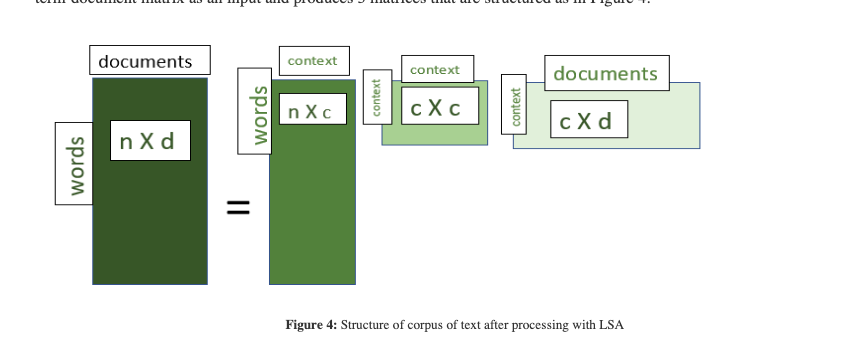
\includegraphics[width=0.2\textwidth]{../images/SVD.png}
    \label{fig:SVD}
\end{figure}
Für eine gegebene Abfrage transformiert LSA diese in einen Pseudo-Dokumentenvektor und berechnet die Ähnlichkeiten mithilfe des SVD-Ergebnis aus der Term-Dokument-Matrix zwischen der Abfrage und dem durchsuchten Dokumenten \cite{SystematicReviewofSemanticAnalysisMethods_2023} .
Im Gegensatz zu präzisen Abgleichmethoden wird die Matrix durch SVD zerlegt, was sie in einen neuen Raum mit niedriger Dimension komprimiert.SVD kann nicht nur die Datenmenge reduzieren, sondern auch die zugrunde liegenden Beziehungen zwischen Begriffen erkennen. 
Aus den oben genannten Gründen, gilt LSA als eine sehr flexible Technik ist und wird oft in der Sprachsuche benutzt wird \cite{TextMiningUsingLatentSemanticAnalysis} .

\begin{enumerate}
    \item \textbf{Fett 1} Nummerierte liste 1
    \item \textit{Kursiv 1} Nummerierte liste 1
    \item Nummerierte liste 1
\end{enumerate}


Eine Matheformel (Satz des Pythagoras):

\[
a^2 + b^2 = c^2
\]

wobei \(a\) und \(b\) die Längen der Katheten eines rechtwinkligen Dreiecks sind, und \(c\) die Länge der Hypotenuse.



\begin{lstlisting}[caption={Pip Update}, label={lst:upgradePip}]
    Python Code Section 1
\end{lstlisting}


'''Deutsche Anführungszeichen''' \ref{label1} referenz Zu Label1 
„Anführungszeichen unten, Anführungszeichen oben“

\ref{bildReferenz} Bild Referenz

\begin{table}[h]
    \centering
    \begin{tabular}{|c|c|}
    \hline
        \textbf{Column1} & \textbf{Column2} \\ \hline
        row1 & row2 \\ \hline
    \end{tabular}
    \caption{Your table caption here}
    \label{table:1}
\end{table}

\newpage
\section{Fazit}
Fazit
\subsection{Ergebnis}
Ergebnis

\subsection{Ausblick}
Ausblick

\newpage


\newpage
\addcontentsline{toc}{section}{Bibliothek}
\markboth{Bibliography}{Bibliography}
\printbibliography[title=Bibliothek]

\newpage
\listoffigures
\addcontentsline{toc}{section}{Abbildungsverzeichnis}%
\markboth{Abbildungsverzeichnis}{Abbildungsverzeichnis}

\newpage
\section*{AI-Verzeichnis}
\markboth{AI-Verzeichnis}{AI-Verzeichnis}
\noindent
\thispagestyle{empty}

 \begin{itemize}
     \item ChatGPT 4o und o1-preview
     \item Consensus AI
     \item Perplexity
     \item DeepL
 \end{itemize}
\newpage

\section*{Ehrenwörtliche Erklärung}
\markboth{hrenwörtliche Erklärung}{hrenwörtliche Erklärung}
\noindent
\thispagestyle{empty}

Wir erklären hiermit ehrenwörtlich:

\begin{enumerate}
	\item dass wir unsere Studienarbeit selbstständig verfasst habe,
	\item dass wir die Übernahme wörtlicher Zitate aus der Literatur sowie die Verwendung der Gedanken anderer Autoren an den entsprechenden Stellen innerhalb der Arbeit gekennzeichnet habe,
	\item dass wir unsere Studienarbeit bei keiner anderen Prüfung vorgelegt habe.
\end{enumerate}
Wir sind uns bewusst, dass eine falsche Erklärung rechtliche Folgen haben wird.
% Etwas Abstand für die Unterschrift
\vspace{2cm}

% Hier kommt die Unterschrift drüber
\begin{tabular}{lp{4em}l} 
 \hspace{5cm}   && \hspace{4cm} \\\cline{1-1}\cline{3-3} 
Ort, Datum     && \studentNameOne 
\end{tabular}

\begin{tabular}{lp{4em}l} 
 \hspace{5cm}   && \hspace{4cm} \\\cline{1-1}\cline{3-3} 
Ort, Datum     && \studentNameTwo
\end{tabular}

\begin{tabular}{lp{4em}l} 
 \hspace{5cm}   && \hspace{4cm} \\\cline{1-1}\cline{3-3} 
Ort, Datum     && \studentNameThree 
\end{tabular}


\newpage
\end{document}